The definitions and notations used throughout this thesis are based on the book of A. Wolksi in Ref.~\cite{wolski2014} unless it is stated otherwise. In this chapter, the basic concepts of accelerator beam physics that are essential for understanding the studies presented here are introduced. The focus is put on the concepts for synchrotrons with proton beams. Additionally, in the last section, the tracking simulation codes used in this work are described.

% Details p.11 Michael schenk
Synchrotrons are circular accelerators where the particles follow a fixed closed-loop path. In a synchrotron, electric fields accelerate the particles while magnetic fields steer and focus them. The magnetic fields are not constant but they vary according to the particles' energy, allowing acceleration and operation in very high (relativistic) energies. The LHC and SPS machines at CERN are synchrotrons like the most of the machines used for High Energy Physics experiments. Usually, in synchrotrons, the beams consist of multiple bunches, longitudinally spaced around the machine, which of course interact with each other. However, these multi-bunch interactions are not relevant to the studies presented in this thesis. Therefore, they are not addressed in the following paragraphs. 

Finally, at this point, it is appropriate to introduce the terms incoherent and coherent effects. Incoherent effects (microscopic approach) affect the individual particles but not the beam as an entity. The incoherent effects cannot be observed by studying the motion of the center of mass (centroid) of the beam. On the contrary, the coherent effects (macroscopic) approach affects the beam as a whole and they can be observed by studying the motion of the centroid.% A) p. 24 M. Schenk
% B) More details in: https://uspas.fnal.gov/materials/09UNM/Unit_8_Lecture_19_Limting_phenomena.pdf

%motion is the microscopic approach where the individual motion of each particle is studied. Coherent motion is the macroscopic approach where the beam is considered as a whole and the motion of the center of mass is studied.

% The section splitting is done here according to Wolski's book.
\section{Motion of charged particles in electromagentic fields}
The motion of a particle with charge $q$ and velosity $\mathbf{v}=(v_x, v_y, v_z)$ moving in an electric field $\mathbf{E}$ and a magnetic field $\mathbf{B}$ is defined by the influence of the Lorentz force: 
\begin{equation}\label{eq:Lorentz_force}
    \mathbf{F} = q(\mathbf{E} + \mathbf{v} \times \mathbf{B}).
\end{equation}
% v is tangential to its path.

At this point, it is appropriate to mention that in this thesis the vectors are denoted in bold font (e.g. $\mathbf{E}$ ). % For the relativistic and ultrarelativistic regime the impacrt of E and B are the same. E = cB. p.44 Wille

In synchrotrons, the electric fields, which are generated by Radiofrequency (RF) cavities, are used for accelerating the beams. The magnetic fields, are used to steer (dipoles) and focus (quadrupoles) and apply corrections (sextupoles, octupoles and higher order multipoles) at the motion of the beam.

\textbf{Reference trajectory and reference particle}\\
The sequence of the various electromagnetic elements around the accelerator ring is called the machine lattice. The ideal path that passes through the center of all the magnets is called the design orbit or the reference trajectory. This reference trajectory (red line Fig.~\ref{fig:coordinate_system}) has circumference $C=2\pi R$ (where $R$ is the radius of the ring) and is predetermined by the construction of the accelerator. 

The particle that follows this trajectory is called the reference particle and has a momentum $p_0$, an energy $E_0$, and a velocity $v_0$. This particle is often called the synchronous particle as it always passes from the center of the RF cavities (assuming constant speed and no losses). %https://indico.cern.ch/event/22574/contributions/475143/attachments/371243/516589/IntroductionToAccelerators.pdf slide 36
For a proton, the reference momentum is given by: $p_0 = \gammarel m_0 v_0$, where $m_p$ is the proton rest mass.

\textbf{Mangetic rigidity}\\
At this point, it is appropriate to introduce the concept of magnetic rigidity, $B_0 \rho$, which is often used in accelerators as a normalisation factor and is a measure of how the charged particles resist bending by a dipolar magnetic field. Assuming that a proton moves only under the influence of a uniform vertical dipole field $\mathbf{B_0}=(0, B_0, 0)$, it would follow a circular path of radius $\rho$ (it will be often referred to as benging radius) which is defined by the Lorentz force (Eq.~\eqref{eq:Lorentz_force}) being equal to the centripetal force, as follows:

\begin{equation}\label{eq:Brho}
    e v_0 B_0 = \frac{\gammarel m_p v_0^2}{\rho} \Rightarrow B_0 \rho = \frac{\gamma_0 m_p v_0}{e} \Rightarrow B_0 \rho = \frac{p_0}{e},
\end{equation}
where $e$ and $m_p$ are the charge and rest mass of a proton respectively, $p_0$ is the reference momentum, and $\gammarel = \frac{1}{\sqrt{1-\beta^2}}$ is the relativistic gamma or Lorentz factor, where $\betarel=v_0/c$ is the relativistic $\beta$ with $c$ being the speed of light. In the ultra-relativistic regime which is the case in the studies presented in this thesis, $\betarel=1$.
% IMPORTANT!!! -->  v_0 = v_z. You explain this in the next paragraph.

If the particle momentum is given in $\mathrm{GeV /c}$ (usuall units in high energy accelerators) then the unit of magnetic rigidity is $\mathrm{T \cdot m}$. 

%- https://uspas.fnal.gov/materials/12MSU/xverse_dynamics.pdf

\textbf{Co-ordinate system}\\
However, the individual particles do not follow the reference trajectory due to small deviations in their initial conditions: an example trajectory is shown in Fig.~\ref{fig:coordinate_system} with the blue line. The co-ordinate system used to describe the individual trajectories of the beam particles around the accelerator is illustrated in Fig.~\ref{fig:coordinate_system} and it is known as Frenet-Serret system.  It consists of the orthogonal co-ordinate system $\Sigma(s) = (\mathbf{e_x}, \mathbf{e_y}, \mathbf{e_z})$ whose origin moves along the reference trajectory (red line) together with the beam. 

The variable $s$ denotes the distance along the reference trajectory. In accelerator physics, $s$ is usually chosen as the independent variable instead of time, $t$.  %why? p.19 https://www.bnl.gov/isd/documents/74289.pdf
Therefore, at any given location $s$ around the ring, the coordinates $(x(s), y(s), z(s))$ give the horizontal, vertical, and longitudinal position of the particle with respect to the origin of the orthogonal moving system $\Sigma$. In the following paragraphs, the dependence of the co-ordinates on the position $s$ along the ring is omitted when possible to facilitate the notation (e.g. x(s) will be denoted as x).

\begin{figure}[!h] % at the directory of ipac22
    \centering         
    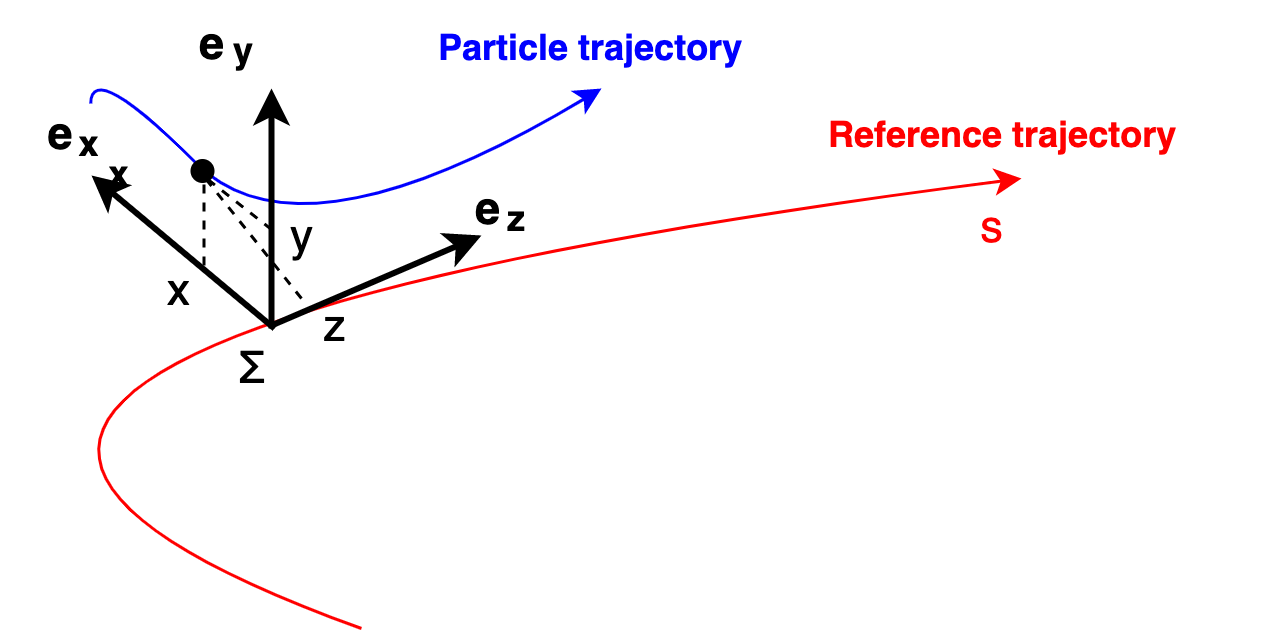
\includegraphics[width=0.8\textwidth]{images/Ch2/coordinates_particle_motion.png}
        \caption{Co-ordinate system used to describe particles motion in a synchrotron. This is a rotating co-ordiante system, with $(\mathbf{e_x, e_y, e_z})$ being the unit vectors, which follows the reference trajectory along the accelerator.}
        \label{fig:coordinate_system}
 \end{figure}


 At any point $s$ along the reference trajectory each particle is represented by the following 6-dimensional vector $(x, x^{\prime}, y, y^{\prime}, z, \delta)$ where:

 \begin{subequations}\label{eq:particle_coordinates}
    \begin{equation}
        x^\prime = \frac{dx}{ds} = \frac{dx}{dt}\frac{dt}{ds} = \frac{v_x}{v_z} =  \frac{p_x}{p_z} \approx \frac{p_x}{p_0},
    \end{equation}    
    \begin{equation}
        y^\prime = \frac{dy}{ds} = \frac{dy}{dt}\frac{dt}{ds} = \frac{v_y}{v_z} =  \frac{p_y}{p_z} 	\approx \frac{p_y}{p_0},
    \end{equation} 
    \begin{equation}
        \delta = \frac{\Delta p}{p_0} = \frac{p-p_0}{p_0},
    \end{equation}
    \begin{equation}
        z = \betarel c (t_0 -t),
    \end{equation}
\end{subequations}

where $p_0$, $\beta_0$ is the momentum of the reference particle and the relativistic $\beta$ as defined in the previous paragraph, $t_0$ is the time  which the reference particle arrives at the location $s$ and $t$ is the time at which the individual particle arrives at the same locaiton. It can be seen, that $\delta$ is the relative momentum offset from the reference particle. In order to avoid a possible misconception it seems appropriate to clarify here, that the longitudinal parameter $z$ indicates the longitudinal offset from the reference particle at the center of the bunch. If $z>0$ ($z < 0$) the corresponding particle reaches earlier (later) than the center of the bunch at an arbitrary reference point. Last, in the ultra-relativistic regime the momentum of the particles in the $\mathbf{e_z}$ direction is much larger than the transvserse ones and almost equals the reference momentum: $p_x, p_y \ll p_z = p_0$. This is why, the $x^\prime$ and $y^\prime$ are basically the normalised momentum with the reference one, $p_0$.

%Furthermore, if the direction of motion of the particle has a small angle with the reference trajectory, the paraxial approximation is valid: $p_x, p_y \ll p_z = p_0$ which means that $x^\prime \approx p_x$ and  $y^\prime \approx p_y$. This approximation is valis for the studies presented in this thesis. \textcolor{red}{$p_0=1$? not clear to me} % ultra relativistic regime, is not mentioned at wolski's book. I wrote it for the p_ 0= 1. but i am not sure.
% p.149 wolski and p.12 Michael schenk

%is the momentum of the reference particle which is given by: $p_0 = \gammarel m_0 v_0$, where $m_0$ is the proton rest mass and
%It can be seen that $x^\prime$ and $y^\prime$ are basically the normalised momenta with the reference momentum $p_0$ and $\delta$ is the relative momentum offset from the reference particle. 

%Initial I have written: Furthermore, the ultra-relativistic regime, the transverse momentum/velocity of a particle is very small comparing to the longitudinal one. Therefore the paraxial approximation is used: $p_x, p_y \ll p_z = p_0 = 1$ which can be applied to simplify Eqs.~\ref{eq:particle_coordinates}. %Or see Andy's explanation for low emittance storage rings: https://cds.cern.ch/record/1982424/plots

To summarize, the motion of the particles is separated in the transverse and longitudinal planes where it is described with the  $(x, x^\prime, y, y^\prime)$ and $(z, \delta)$ co-ordinates respectively. As an example the co-ordinates of the reference particle are $(x=0, x^\prime=0, y=0, y^\prime = 0, z=0, \delta=0 \ (p_z=p_0))$.

Last, $(x, y, z)$ are expressed in meters, $(x^\prime, y^\prime)$ in radians while $\delta$ is dimensionless.

\section{Single-particle beam dynamics}
In this first section, the interactions between the particles within a bunch are neglected, hence the term single-particle beam dynamics. 

\textbf{Two-dimensional complex fields}\\
As already discussed, the motion of the charged particles inside a circular accelerator is controlled by magnetic fields. In this thesis, the magnets are considered purely transverse elements. Their effect is therefore described with two-dimensional multipole fields, acting in the horizontal and vertical planes\footnote{Examples of three-dimensional treatment can be found in~\cite{wolski2014, Beth:889480}. However, the two-dimensional treatment is most often used in accelerator physics as it provides a good description for the majority of the magnetic elements.}. % Wolski Ch1.3, p.33

The description of two-dimensional magnetic fields in accelerator physics is discussed using the concept of multipole expansion and is expressed as a complex quantity. The complex quantity it allows to describe a two-dimensional field in $(x,y)$ space (to be compatible with the co-ordinates used for describing the particle's trajectory as discussed in the previous section). Therefore, the magnetic field around the beam is expressed as follows~\cite{wolski2014}: 
\begin{equation}\label{eq:mult_expansion} % Andy Eq.1.29 + M Schenk Eq.2.2
    B_y(x,y) + i B_x(x,y) = \sum_{n=1}^{\infty} C_n (x+i y)^{n-1},
\end{equation} % principle of superposition 
where $n$ indicates the order of the field component: $n$=1 for a dipole (steering), $n$=2 for quadrupole (focusing (chromticity correction), $n$=4 for octupole (error or field correction) etc. $C_n=(b_n +i \alpha_n)$ is a complex constant which denotes the strength and orientation of the multipole field. The coefficients $b_n=\frac{1}{(n-1)!} \frac{\partial^{n-1}B_y}{\partial x^{n-1}}$ and $\alpha_n=\frac{1}{(n-1)!} \frac{\partial^{n-1}B_x}{\partial x^{n-1}}$ denote the strength of a normal and skew (normal multipole rotated by $\pi/2(n-1)$) multipole respectively in units of $\mathrm{T/m^{n-1}}$.
% Equations for coefficients, sofia's thesis Eq.(2.29) p. 23: https://cds.cern.ch/record/2743602/files/CERN-THESIS-2020-169.pdf

Usually, in accelerator physics the values of the multipole strengths are quoted normalised to the magnetic rigidity as defined in Eq.~\eqref{eq:Brho} and are denoted by:
\begin{equation}\label{eq:kn}
    k_n = \frac{b_n}{B_0 \rho},
\end{equation}
and is expressed in untis of  $\mathrm{T/m^{n}}$. This is the convention that will be used in this thesis.

\subsection{Transvserse motion}
In the transverse plane the motion is orthogonal to the reference trajectory (see Fig.~\ref{fig:coordinate_system}) and its co-ordinates are $(x, x^\prime, y, y^\prime)$. For the discussion on the transverse beam dynamics, the $(x, x^\prime)$ and $(y, y^\prime)$ co-ordinates will be both described by $(u, u^\prime)$ when possible to facilitate the notation.

\subsubsection{Linear dynamics}
Here the transverse motion of a particle moving the two-dimensional fields described in Eq.~\eqref{eq:mult_expansion} is discussed. For now the discussion is limited only in dipolar and quadrupolar components ($n=1$ and $n=2$) hence the name linear dynamics. Dipoles and quadrupoles are considered the basic magnetic elements, as in the absence of magnetic errors or momentum deviations between the particles they are sufficient to create a synchrotron. 

As mentioned above, the particles (but the reference one) transversely  oscillate around the reference trajectory. This motion, through an arbitrary periodic sequence of dipoles and quadrupoles is called betatron motion and can be described with the following equations of motion~\cite{Lee:1425444}:
% also sofia's thesis Eq.(2.37)

\begin{equation}\label{eq:transverse_eq_x}
    x^{\prime \prime} - \frac{\rho+x}{\rho^2} = - \frac{B_y}{B_0 \rho} \frac{p_0}{p} \left (  1+ \frac{x}{\rho} \right )^2, 
\end{equation}

\begin{equation}\label{eq:transverse_eq_y}
    y^{\prime \prime} = \frac{B_y}{B_0 \rho} \frac{p_0}{p}  \left (  1+ \frac{x}{\rho} \right )^2, 
\end{equation}

where $s$ is the distance along the reference trajectory, $B_0 \rho$ and $\rho$ the magnetic rigidity and radius as defined in Eq.~\eqref{eq:Brho},  $B_y, B_x$ the transverse magnetic fields of Eq.~\eqref{eq:mult_expansion}, and $p_0$ the reference momentum.

For on-momentum particles ($\delta = 0$) the above betatron equations of motion are simplified to the equation of harmonic oscillator (but with an $s$ dependent strength $K_u(s)$), named the Hill's equation~\cite{Lee:1425444}:

\begin{equation}\label{eq:Hills_equation_1}
    u^{\prime \prime}(s) + K_u(s) u(s) = 0,
\end{equation}

where $u=(x,y)$ and:

 \begin{equation}\label{eq:Hills_equation_2}
    K_u(s) = \begin{dcases}
        \frac{1}{\rho(s)}+k_1(s), & u=x \\
        -k_1(s), & u=y 
    \end{dcases}
\end{equation}

with $k_1(s)$ being the normalised quadrupole strength. It should be noted that for Eq.~\eqref{eq:Hills_equation_1} it is assumed that the motion in horizontal and vertical plane are independent (uncoupled).

Equation~\eqref{eq:Hills_equation_1} looks like the second-order differential equation of an harmonic oscillator, but the constant $K_u$ depends on the variable $s$. For a circular accelerator $K_u$ is periodic: $K_u(s+C_0)=K_u(s)$, where $C_0$ is the periodicity of the accelerator and real-valued. The general solution of the Hill's equations is:
\begin{equation}\label{eq:Hills_solution}
    u(s) = A w(s) \cos{(\psi_u(s)+\psi_{u,0})},
\end{equation}
where $A$ and $\psi_{u,0}$ the integration constants and $w(s)$ and $\psi_u(s)$ are the amplitude and betatron phase functions, which are periodic functions with the same periodicity as $K_u$.

By inserting Eq.~\eqref{eq:Hills_solution} in Eq.~\eqref{eq:Hills_equation_1} and after performing a series of computations which are shown in detail in Appendix~\ref{app:betatron_equations_solutions} it is found that the amplitude and phase functions fulfill the following equations: 
%Combination slide 27-28 of yiannis notes:  https://yannis.web.cern.ch/teaching/transverse.pdf and federicos thesis (p.11): https://cds.cern.ch/record/1481835/files/CERN-THESIS-2005-082.pdf

\begin{equation}\label{eq:phase_functions}
    w^{\prime \prime}_u + K_u(s) w(s) -\frac{1}{w_u(s)^3} = 0, 
\end{equation}
where:
\begin{equation}\label{eq:phase_function}
    \psi^{\prime}_u(s) = \frac{1}{w_u(s)^2} \Rightarrow \psi_u(s) = \int_{s_0}^{s} \frac{ds}{w_u(s)^2}
\end{equation}
The above equations are called the betatron envelope and phase equations.

\textbf{Courant-Snyder parameters}\\
At this point it is appropriate to introduce the betatron or twiss or Courant-Snyder or twiss parameters:% frpom Yiannis notes: https://yannis.web.cern.ch/teaching/transverse.pdf
\begin{subequations}\label{eq:twiss_func}
    \begin{equation}
        \beta_u(s) = w_u(s)^2,
    \end{equation}    
    \begin{equation}
       \alpha_u(s) = -\frac{1}{2} \beta^{\prime}_u(s),
    \end{equation} 
    \begin{equation}
       \gamma_u(s) = \frac{1+\alpha_u(s)^2}{\beta_u(s)},
    \end{equation}
\end{subequations}
with $\beta^{\prime}_u(s) = d\beta_u(s)/ds$.

The betatron phase advance from Eq.~\eqref{eq:phase_function} can be re-written using the beta twiss function as:
\begin{equation}\label{eq:phase_advance_definition_with_twiss}
    \psi_u(s)= \int_{s_0}^{s} \frac{ds}{\beta_u(s)}.
\end{equation}
%As $K_u(s)$ is a periodic function, the two independent solutions of the second order differential Eq.~\eqref{eq:Hills_equation_1} can be expressed using the Floquet theorem~\cite{Floquet1883} as follows (see Appendix A, Sec. I.5 in Ref.~\cite{Lee:1425444}):

%\begin{equation}\label{eq:Floquets_solutions}
%    u(s) = a_u w(s)e^{i \psi_u (s)}, \ u^*(s) = a_u w(s)e^{-i \psi_u (s)},
%\end{equation}

%where $\alpha_u$ is a constant, and $w(s)$ and $\psi(s)$ are the amplitude and betatron phase functions and $u^*(s)$ is the complex conjugate of $u(s)$. 
%$K_u(s)$ is real-valued, therefore the amplitude and phase functions fulfill the following equations: % Lee Eq.(2.38), % p.250 widerman

% If you want to see how you go from Eq.(2.10) to Eq.(2.11) see also Yiannis notes (p.27-28): https://yannis.web.cern.ch/teaching/transverse.pdf

\textbf{Betatron tune}\\
Another important quantity in accelerator physics is the betatron tune or just tune of the machine, $Q_u$, which is the phase advance for one complete revolution around the machine devided by $2\pi$:
\begin{equation}\label{eq:betatron_tune}
    Q_u = \frac{\psi_u(s+C)-\psi_u(s)}{2\pi} = \frac{1}{2\pi} \oint_C \frac{ds}{\beta_u(s)},
\end{equation}
where $C$ the circumference of the machine. As it can be seen, the tune also represents the number of betatron oscillations that a particle undergoes during one full revolution around the machine. 

The tune of the individual particles may vary due to effects such as the chromaticity, the detuning with their transverse amplitude and collective forces (e.g. impedance) that will be discussed in the following paragraphs. The horizontal and vertical tune of the reference particle will be referred to as the bare tune and define what is called the working point of the machine, $(Q_{x0}, Q_{y0})$. 

\textbf{Matrix formalism}\\
% w and psi are also solutions. now we write it in matrix notation
Knowing the lattice (element per element structure of the accelerator) the solutions $w_u(s)$ and $\psi_u(s)$ of the Hill's equation can be also described using a matrix formalism as follows:

\begin{equation}\label{eq:matrix_formalism_intro}
   \begin{pmatrix}
    u\\ 
    u^\prime
    \end{pmatrix}_{s_1} = M_u (s_1 |  s_0) \begin{pmatrix}
    u\\ 
    u^\prime
    \end{pmatrix}_{s_0},
\end{equation}

where $u=(x,y)$. The transfer matrix from the position $s_0$ to the $s_1$, $M_u (s_1 |  s_0)$, equals to~\cite{Lee:1425444}: %Eq.(2.42) lee

\begin{equation}\label{eq:linear_transfer_matrix}
    \begin{split}
    M_u (s_1 |  s_0) &= \begin{pmatrix}
        \sqrt{\frac{\beta_u(s_1)}{\beta_u(s_0)}} (\cos{\Delta \psi_u}+\alpha_u (s_0) \sin{\Delta \psi_u}) & \sqrt{\beta_u(s_0)\beta_u(s_1)}\sin{\Delta \psi_u} \\ 
         - \frac{1+\alpha_u(s_0) \alpha_u(s_1)}{\sqrt{\beta_u(s_0) \beta_u(s_1)}} \sin{\Delta \psi_u}+ \frac{\alpha_u(s_0) - \alpha_u(s_1)}{\sqrt{\beta_u(s_0) \beta_u(s_1)}} \cos{\Delta \psi_u} & \sqrt{\frac{\beta_u(s_0)}{\beta_u(s_1)}} (\cos{\Delta \psi_u}+\alpha_u(s_1) \sin{\Delta \psi_u})
        \end{pmatrix} \\ 
        &=\begin{pmatrix}
            \sqrt{\beta_u(s_1)} & 0 \\
            -\frac{\alpha_u(s_1)}{\sqrt{\beta_u(s_1)}}& \frac{1}{\beta_u(s_1)}
            \end{pmatrix} \begin{pmatrix}
            \cos{\Delta \psi_u} & \sin{\Delta \psi_u} \\
            -\sin{\Delta \psi_u}& \cos{\Delta \psi_u}
            \end{pmatrix} \begin{pmatrix}
            \frac{1}{\sqrt{\beta_u(s_0)}} & 0 \\
            \frac{\alpha_u(s_0)}{\sqrt{\beta_u(s_0)}} & \sqrt{\beta_u(s_0)}
            \end{pmatrix},
    \end{split}
\end{equation}
where $\Delta \psi_u = \psi_u(s_1)-\psi_u(s_0)$ is the betatron phase advance between the two locations while $\alpha_u(s_i)$ and $\beta_u(s_i)$ are the Courant-Snyder parameters at the location $s_i$, where $i=(0,1)$. The convinient transfer matrix apporoach will be extrensively used throught this thesis to study the motion of the particles in the accelerator lattice.

\textbf{Action angle variables and phase space ellipse}\\
The solution of equation of motion (Eq.~\eqref{eq:Hills_equation_1}) can alternatively be expressed in action-angle co-ordinates $(J_u, \psi_u)$ as follows:
\begin{equation}\label{eq:position_action_anlge}
    u(s) = \sqrt{2 \beta_u(s) J_u} \cos{(\psi_u(s))}.
\end{equation} 
By differantion the divergence $u^\prime$ is written as:
\begin{equation}\label{eq:divergence_action_anlge}
    u^\prime(s) = - \sqrt{\frac{2 J_u}{\beta_u(s)}} (\sin{(\psi_u(s))}+\alpha_u(s)\cos{(\psi_u(s))}),
\end{equation} 
where $\beta_u(s), \alpha_u(s)$ the twiss parameters as defined in Eq.~\eqref{eq:twiss_func}, $\psi_u(s)$ the betatron phase as defined in Eq.~\eqref{eq:phase_function} and $J_u$ is an integration constant which is defined by the initial conditions. % D. Amoriom p. 12

The action, $J_u$ is an invariant of the motion and can be written in terms of the twiss parameters as: % A. Wolski p.137
\begin{equation}\label{eq:action_definition}
    J_u = \frac{1}{2} (\gamma_u(s) u^2(s) + 2 \alpha_u(s) u(s) u(s)^\prime + \beta_u(s) u^{\prime 2}(s)) = \mathrm{constant}.
\end{equation}

The trajectory of each individual particle can be plotted in phase space $(u, u^\prime)$ at a given position $s$ in the ring turn after turn. In phase space the particle's path is an ellipse whose shape and orientation are determined by the twiss parameters at the position $s$. This ellipse, named phase space or Courant-Snyder ellipse, is illustrated in Fig.~\ref{fig:phase_space_ellipse} and it has an area $2\pi J_u$. It is worth mentioning, that the ellipse's size is different for each particle as it depends on their individual actions, $J_u$ i.e. their individual initial conditions. The origin of the ellipse is the closed orbit which is basically the reference trajectory and is also shown in the plot.

\begin{figure}[!h] % at the directory of ipac22
    \centering         
    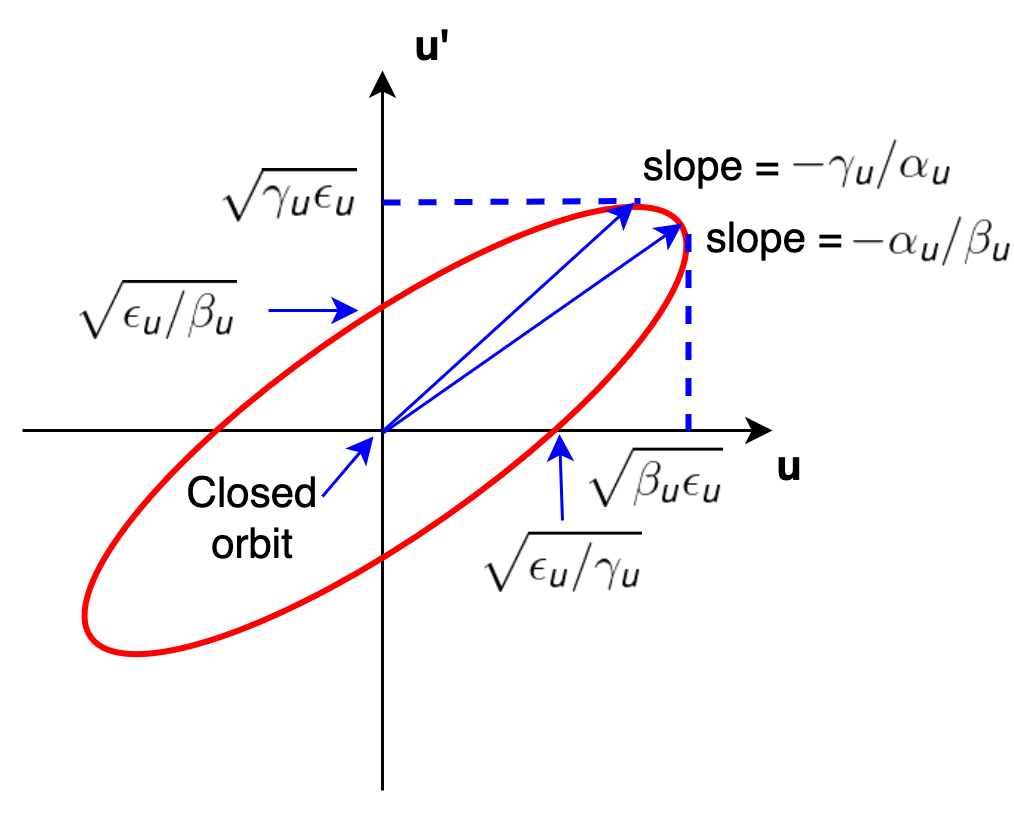
\includegraphics[width=0.6\textwidth]{images/Ch2/phase_space_ellipse.png}
        \caption{Phase space co-ordinates $(u, u^\prime)$ turn by turn, for a particle moving along the ring but at a particular position $s$ which is characterised by the following twiss parameters $[\alpha_u(s), \beta_u(s), \gamma_u(s)]$. For the plotting, the dependence on the $s$ parameter has been omitted.}
        \label{fig:phase_space_ellipse}
 \end{figure}

 \textbf{Normalised phase space}\\  %Federicos thesis 2.3.1 and sondre eq. 2.21a
 Often in accelerator physics it is useful to transform the transverse phase space ellipse to a normalised phase space circle, where the motion is equivalent with the one of the harmonic oscillator. % Wiedemman p.235 
 In the normalised phase space the co-ordinates $(u, u^\prime)$ are normalised with the twiss parameters $(\alpha_u, \beta_u)$ for the particular location $s$ around the ring, as follows~\cite{Wiedemann:1083415}: % widerman p.235, eq.8.92-8.93
 \begin{equation}\label{eq:normalised_coordinates_un}
     u_N(\phi) = \frac{u(s)}{\sqrt{\beta_u(s)}},
 \end{equation}
\begin{equation}\label{eq:normalised_coordinates_un_prime}
     u^\prime_N(\phi) = \frac{d u_N}{d \phi} = \sqrt{\beta_u(s)} u^\prime(s) + \frac{\alpha_u(s)}{\beta_u(s)}u(s),
 \end{equation}
 % The normalised transformation can also be found in Yiannis notes in the link below: https://yannis.web.cern.ch/teaching/transverse.pdf
where $\phi = \frac{\psi_u}{Q_u}$. It can be seen that the indipendent variable in the normalised co-ordinates is the phase advance (normalised with the betatron tune), $\phi$, instead of the location $s$ along the ring. % p.12 in the following link: https://cds.cern.ch/record/409584/files/thesis-99-070_Chapter1.pdf
Both of the normalised co-ordinates, $(u_N, u_N^\prime)$ are expressed in units of $m^{1/2}$.

Combining Eq.~\eqref{eq:action_definition}, Eq.~\eqref{eq:twiss_func}, Eq.~\eqref{eq:normalised_coordinates_un} and Eq.~\eqref{eq:normalised_coordinates_un_prime} the action variable can also be written as:
\begin{equation}\label{eq:action_normalised_coordinates}
    J_u = \frac{1}{2} (u_N^2+u_N^{\prime 2}).
\end{equation}
% Plotting in p.4 of: http://www.toddsatogata.net/2013-USPAS/2013-01-23-NonlinearDynamicsNotes.pdf
The phase space in normalised co-ordinates is shown in Fig.~\ref{fig:phase_space_circle_normalised}.
\begin{figure}[!h] % at the directory of ipac22
    \centering         
    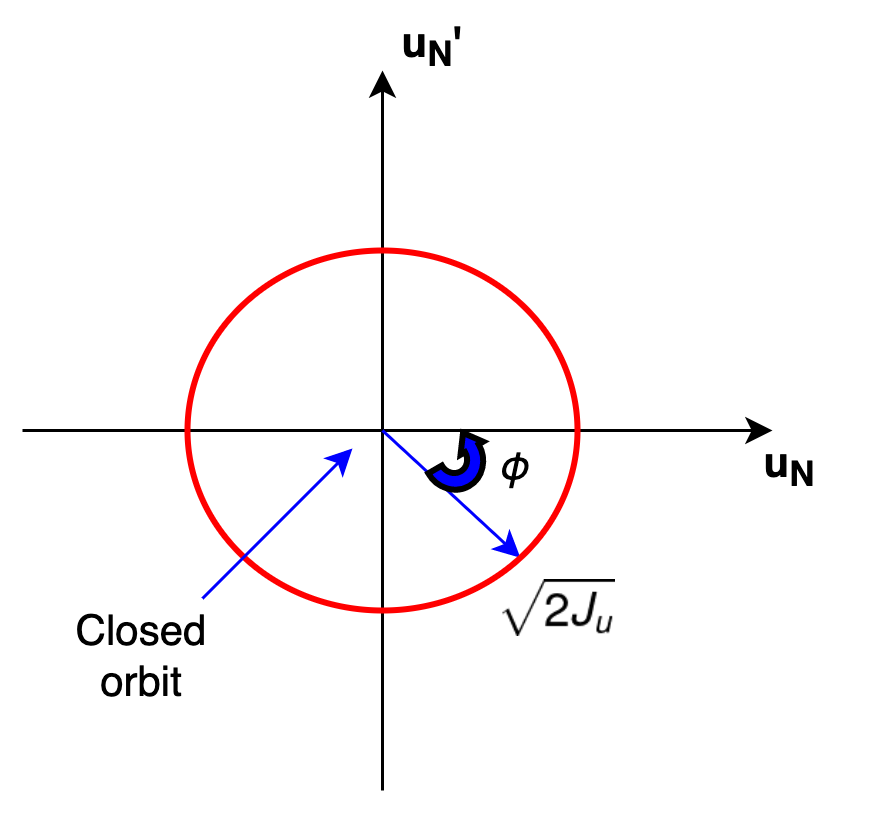
\includegraphics[width=0.6\textwidth]{images/Ch2/phase_space_normalised.png}
        \caption{Normalised phase space for a particle moving along the accelerator but for a particular position $s$. The particle moves turn by turn in a circle of radius $\sqrt{2J_u}$.}
        \label{fig:phase_space_circle_normalised}
 \end{figure}

The distribution of actions is an exponential distribution \textcolor{red}{How do I prove this?} which implies that its mean equals its standard deviation. This property will be used for computations in the following chapters. % Actually, this property is used in the appendix for the computation of the rms tune spread.

%From Eq.~\eqref{eq:action} we write:
%\begin{equation}\label{eq:Jy_exp_distr}
%    e^{-J/\epsilon} = e^{(-x^2/2\epsilon - px^2/2\epsilon)}
%\end{equation}
%From this equation it can be seen that the actions follow an exponential distribution. 

\textbf{Transvserse emittance}\\
Up to now, the twiss parameters were used to describe the dynamics of single particles. However, they also describe the distribution of the particles within a bunch. The statistical average of $u^2$ over all particles at a given point $s$ along the reference trajectory, from Eq.~\eqref{eq:position_action_anlge} equals to~\cite{wolski2014}:
\begin{equation}\label{eq:statistical_average_position}
    \langle u^2(s) \rangle = 2 \beta_u(s) \langle J_u \cos^2{\psi_u(s)} \rangle.
\end{equation}
Assuming, that the angle and action variables are uncorrelated and that the angle variables are uniformly distributed: % angles uniformly distributed from (0,2pi)
\begin{equation}\label{eq:mean_u_zerp}
    \langle u(s) \rangle = 0,
\end{equation}
and then Eq.~\eqref{eq:statistical_average_position} becomes:
\begin{equation}\label{eq:emittance_definition_1}
    \langle u^2(s) \rangle = \beta_u(s) \epsilon_u,
\end{equation}
where
\begin{equation}\label{eq:geom_emittance_action}
    \epsilon_u=\langle J_u \rangle
\end{equation}
is the geometric emittance of the bunch. Considering the same assumption Eq.~\eqref{eq:position_action_anlge} and  Eq.~\eqref{eq:divergence_action_anlge} results to:
\begin{equation}\label{eq:u_uprime_eq_1}
    \langle u(s) u^\prime(s) \rangle = - \alpha_u(s) \epsilon^{\mathrm{geom}}_u,
\end{equation}
\begin{equation}\label{eq:u_uprime_eq_2}
    \langle u^{\prime 2}(s) \rangle = \gamma_u(s) \epsilon^{\mathrm{geom}}_u.
\end{equation}

Combining the above equations, the geometric emittance is expressed in terms of the particles' distribution as:

\begin{equation}\label{eq:geometric_emittance_v2}
    \epsilon^{\mathrm{geom}}_u = \sqrt{\langle u^2(s) \rangle \langle u^{\prime 2}(s) \rangle- \langle u (s)u^{\prime}(s) \rangle ^2}
\end{equation}

which, for $\langle u(s) \rangle=0$ (Eq.~\eqref{eq:mean_u_zerp}), equals the covariance or Sigma matrix of the particles' distribution (Eq~\eqref{eq:Sigma_matrix}):

\begin{equation}\label{eq:Sigma_matrix}
    \Sigma = \begin{pmatrix}
        \langle u^2(s) \rangle & \langle u(s) u^\prime(s) \rangle \\ 
        \langle u(s) u^\prime(s) \rangle & \langle u^{\prime 2}(s) \rangle 
        \end{pmatrix}  = \begin{pmatrix}
            \sigma_u^2(s) & \langle u(s) u^\prime(s) \rangle \\ 
            \langle u(s) u^\prime(s) \rangle & \sigma_{u^{\prime 2}(s)} 
            \end{pmatrix} 
\end{equation}

The square root of the top-left element of the Sigma matrix, $\sigma_u$, is defined as the rms beam size and is also a variable that is used extensively in accelerator physics. The definition of rms and of others of the statistical analysis can be found in Appendix~\ref{ch:app_A}.

Figure~\ref{fig:phase_space_emittance} provides a visualisation of the concepts of emittance and rms beam size. It shows the phase space of a transverse Gaussian bunch along with the histograms of the $u$ (top) and $u^\prime$ (right) variables at a particular point $s$ along the ring. Each particle follows its individual ellipse (of different sizes but with the same orientation) depending on its initial conditions. The rms beam size, $\sigma_u$, and the rms normalised momentum spread, $\sigma_{u^\prime}$, are shown in the top and right histograms of Fig.\ref{fig:phase_space_emittance} with the blue vertical lines. This corresponds to the area of the ellipse enclosed in the blue line in the phase space plot and equals the rms or geometric emittance, $\epsilon^{\mathrm{geom}}_u$ , as defined in Eq.~\eqref{eq:geometric_emittance_v2}.

\begin{figure}[!h] 
    \centering         
    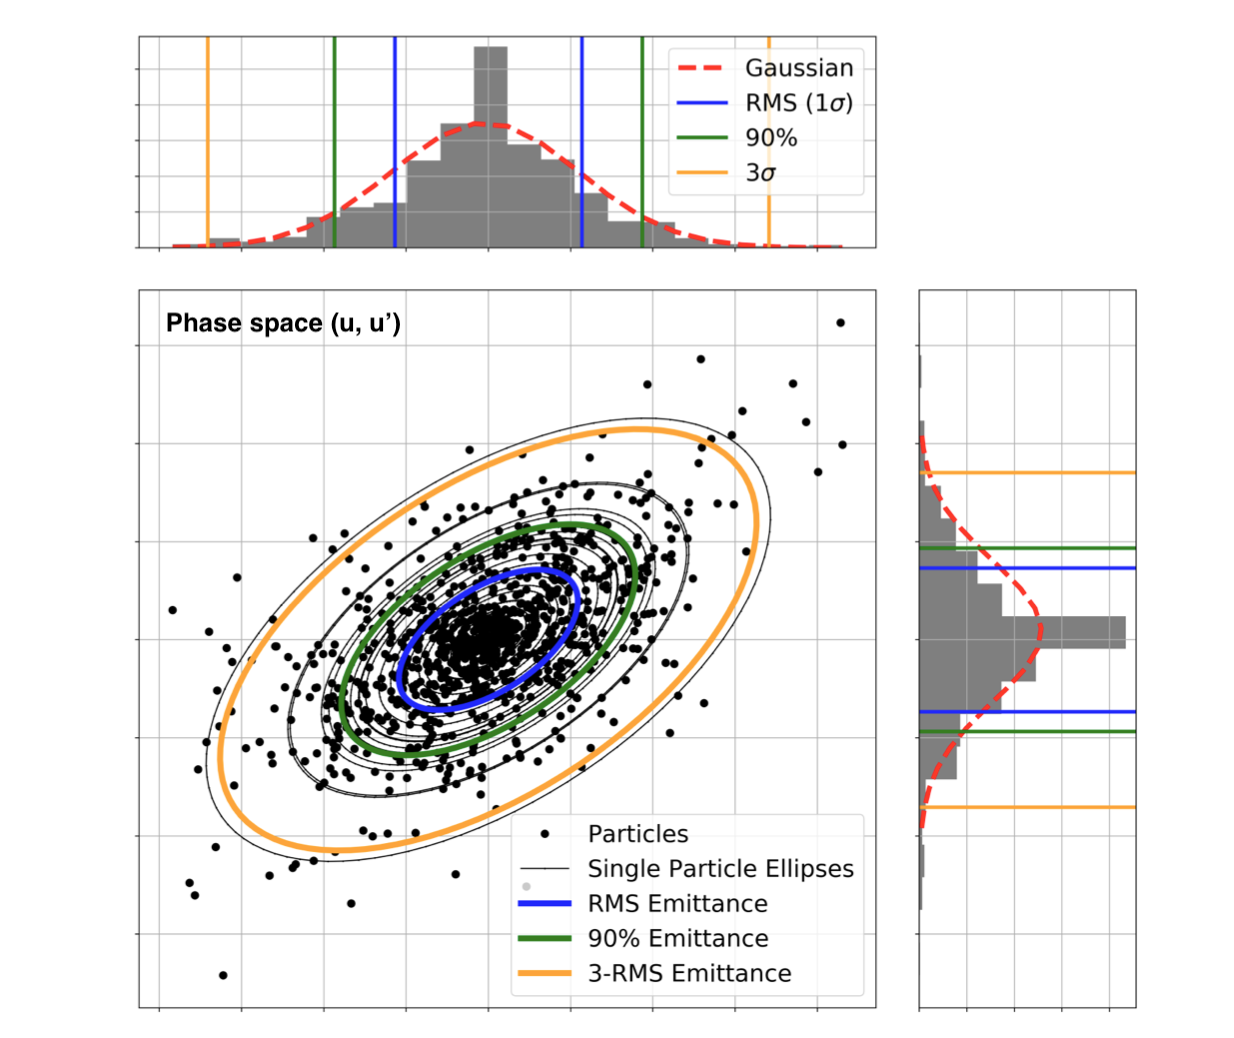
\includegraphics[width=0.9\textwidth]{images/Ch2/transverse_phase_space_emittance.png}
        \caption{Transverse phase space of a Gaussian bunch. The figure is a courtesy of Tirsi Prebibaj~\cite{tirsi_thesis_presentation}.}
        \label{fig:phase_space_emittance}
 \end{figure}

It should be noted, that there are also other conventions to define the emittance such as the 90$\%$ emittance (green lines in Fig.~\ref{fig:phase_space_emittance}) or the 3-sigma emittance (yellow lines in Fig.~\ref{fig:phase_space_emittance}). However, here the term geometric emittance will refer to the rms geometric emittance.

According to Liouville’s theorem~\cite{wolski2014}, considering that there are no interactions between the particles and that the energy of the beam is not changing, the geometric emittance remains constant and therefore is an invariant of bunch motion (similarly to the action $J_u$ for the single-particle motion). The geometric emittance does not remain constant during acceleration, instead the normalised emittance is defined as:
\begin{equation}\label{eq:normalised_emittance}
    \epsilon_u = \beta_0 \gamma_0 \epsilon^{\mathrm{geom}}_u
\end{equation}
The normalised emittance is conserved during acceleration and therefore it is most often used in accelerator physics. It is highlighted here, that throughout this thesis the term "emittance" will refer to the rms normalised emittance.

It is worth commenting here, that for the simulation studies presented in this thesis, the emittance is computed using the statistical definition introduced in Eq.~\eqref{eq:geometric_emittance_v2}. In the experimental studies, the emittance is obtained with a Gaussian fit of the bunch distribution, to obtain its $\sigma$. This process is explained extensively in Chapter~\ref{Ch:2018_analyisis}. For that case, the normalised emittance is obtained from the following formula which is obtained form Eq.~\eqref{eq:emittance_definition_1}, Eq.~\eqref{eq:Sigma_matrix} and Eq.~\eqref{eq:normalised_emittance}:

% For a Gaussian beam distribution the normalised beam emittance it applies:
\begin{equation}\label{eq:emit_from_beam_size}
    \epsilon_{u} = \frac{\sigma_u(s)^2}{\beta_u(s)} \beta_0 \gamma_0,
\end{equation}

where $\sigma_u(s)$ is the rms beam size, $\beta_u(s)$ is the beta function, at specific location $s$ along the accelerator and $\beta_0, \gamma_0$ are the relativistic parameters. 

It should be highlighted that the emittance definitions of Eq.~\eqref{eq:geometric_emittance_v2} (after normalisation with the relativistic parameters) and of Eq.~\eqref{eq:emit_from_beam_size} are equivalent.

Finally, despite Liouville’s theorem in a real accelerator there are various phenomena that change the emittance such as~\cite{Buon:216507}: scattering on residual gas, intra-beam scattering, beam-beam scattering, stochastic or electron cooling, synchrotron radiation emission, filamentation due to non-linearities of the machine, space charge and noise effects. The studies in this thesis focus on the emittance growth due to noise effects (discussed in more details in Chapter~\ref{Ch:CC_noise_theory}).

\textbf{Off-momentum effects - dispersion}\\
Up to now, the discussion was limited to on-momentum particles $\delta=0$: their momentum equals the reference momentum, $p_0$. In a more realistic beam, however, the momentums of the individual particles are spread around the reference one $p_0$ and this is expressed with the longitudinal co-ordinate $\delta=(p-p_0)/p_0$ defined in Eq.~\eqref{eq:particle_coordinates}. As an example, in the SPS machine, which is of interest for this thesis, $\delta$ is in the order of magnitude of $10^{-4}$ to $10^{-3}$.

The off-momentum particles experience different forces than the reference particle when passing through the magnetic fields in an accelerator. Here their motion through the dipole magnets which leads to dispersion effects is discussed. 

Particles with $\delta < 0$ ($\delta>0$) are deflected stronger (less) by the dipole magnets than the reference particle due to lower (higher) magnetic rigidity. Therefore, they travel along the accelerator performing betatron oscillations not around the reference trajectory but around a different closed orbit as illustrated in Fig.~\ref{fig:closed_orbit_Dx} which depends on their momentum spread $\delta$. This dependence of the closed orbit on the momentum offset of the particle is called dispersion.

\begin{figure}[!h] % 
    \centering         
    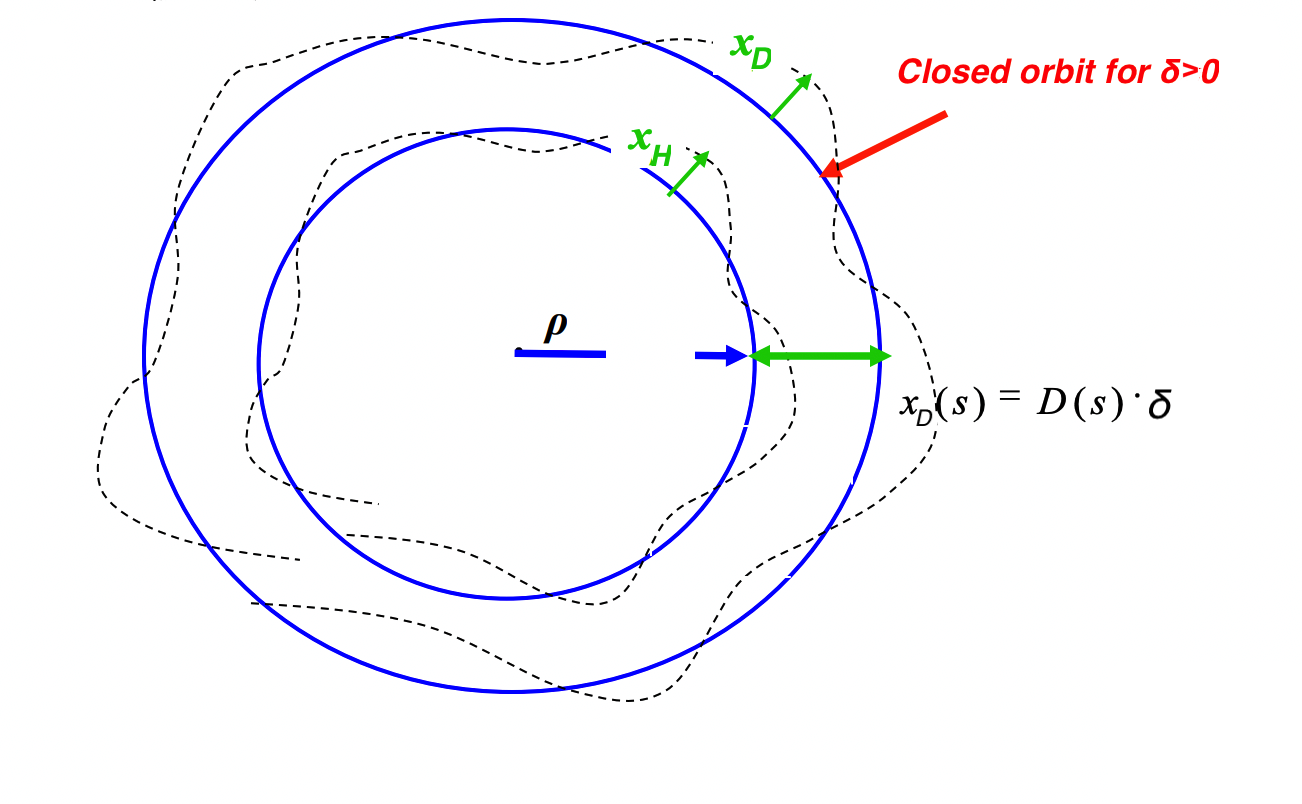
\includegraphics[width=0.6\textwidth]{images/Ch2/closed_orbit_dispersion.png}
        \caption{The closed orbit and the betatron oscillations around it in the presence of dispersion~\cite{Holzer_summer_students_introduction}}
        \label{fig:closed_orbit_Dx}
 \end{figure}

The equation of motion for the off-momentum particles is:
\begin{equation}
    x^{\prime \prime}(s) + K_x(s)x(s) = \frac{1}{\rho(s)} \delta,
\end{equation}
with the following solution:
\begin{equation}
    x(s) = x_H(s) + D_x(s)\delta,
\end{equation}
where $x_H(s)$ is the homogeneous solution shown in Eq.~\eqref{eq:position_action_anlge} and $D_x(s)$ is the dispersion function which can be expressed as:
\begin{equation}\label{eq:dispersion_function}
    D^{\prime \prime}_x(s) + K_x(s)D_x(s) = \frac{1}{\rho(s)}.
\end{equation}

%Its solution is the sum of the solutions of homogeneous (for $\delta=0$) and of the inhomogeneous ($\delta \neq 0$) equation:
%\begin{equation}
%    x(s) = x_H(s) + x_I(s) = x_H(s) + D_x(s)\delta,
%\end{equation}

% which is defined as:
%\begin{equation}\label{eq:dispersion_function}
%   D_x(s) = \frac{x_I(s)}{\delta}
%\end{equation}

The dispersive contribution can be added to the transfer matrix introduced in Eq.~\eqref{eq:matrix_formalism_intro} as follows:
\begin{equation}\label{eq:matrix_formalism_dispersion}
    \begin{pmatrix}
     x\\ 
     x^\prime
     \end{pmatrix}_{s_1} = M_x (s_1 |  s_0) \begin{pmatrix}
     x\\ 
     x^\prime
     \end{pmatrix}_{s_0} + \delta \begin{pmatrix}
        D_x\\ 
        D_x^\prime
        \end{pmatrix}_{s_0}.
 \end{equation}
%The transfer matrix $M$ can be re-written such as it inclyyded, alide 14 in presentation v2 below:

% 1. Definition of D: https://yannis.web.cern.ch/teaching/transverse.pdf
% 2. Definition of D prime: https://indico.cern.ch/event/847209/contributions/3558973/attachments/1932901/3201996/AccPhys_Lect7_MomEff.pdf

 From the discussion above, it becomes clear that the dispersion couples the longitudinal with the horizontal motion. The dispersion effects are discussed here only for the horizontal plane due to the fact that (as stated already) only vertical dipolar fields are considered. As an example, the rms horizontal dispersion of the SPS machine is about 1.8\,m (model value). %/Users/nataliatriantafyllou/PhD_projects/exploring_SPS/madx_studies/optics_new_seq_after_LS2/output/twiss_thin_elements
 
 At this point, it is appropriate to mention that only the model vertical dispersion equals zero. In a real machine, vertical dispersion can be introduced by sources such as the steering errors of the dipole or quadrupole magnets~\cite{Wolski_uspas}. As an example, the rms vertical dispersion in the SPS machine is measured to be about 10\,cm.

Finally, in the presence of dispersion the normalised beam emittance (Eq.~\eqref{eq:emit_from_beam_size}) becomes:
\begin{equation}\label{eq:emit_from_beam_size_Du}
    \epsilon_{u} = \frac{\sigma_u(s)^2 - \delta^2 D_u^2(s)}{\beta_u(s)} \beta_0 \gamma_0,
\end{equation}
where $\sigma_u(s)$ is the rms beam size, $\beta_u(s)$ is the beta function, $D_u(s)$ is the dispersion fat a specific location s along the accelerator, $\delta$ is the momentum spread and $\beta_0, \gamma_0$ the relativistic parameters.

Additionally, the off-momentum particles receive different focusing due to gradient errors in the quadrupoles. This effect is known as chromaticity and is discussed in detail in the next subsubsection which focuses on non-linear beam dynamics.

\subsubsection{Non-linear dynamics}
Up to now, only linear elements (dipoles and quadrupoles) were considered as in theory they are sufficient to create a synchrotron. However, in a real machine non-linearities are also present due to factors such as imperfections in the magnets field and alignment, particles' momentum spread, and higher order magnets (sextupoles, octupoles, etc). Here, the preceding discussion is expanded to include the non-linear beam dynamics. The discussion is limited in the two effects that are important for the work presented in this thesis: the chromaticity and the detuning with transverse amplitude.

\textbf{Chromaticity}\\
We define the chromaticity as the variation of the betatron tune $Q_u$ with the relative momentum deviation delta. This is a result of the fact that particles with $\delta < 0$ ($\delta > 0$) recieve a weaker (stronger) focusing strength from the quadrupoles due to their larger magnetic rigidity. The tune shift introduced by the chromaticity for each particle (incoherent), $ \Delta Q_u (\delta)= Q_u - Q_{u0}$, is: % M. Schenk p.49

%The tune shift introduced by the chromaticity is: % M. Schenk p.49

\begin{equation}\label{eq:chromatic_tune_shift_up_to_order_m}
   \Delta Q_u (\delta) = \sum_{n=1}^m \frac{1}{n!} Q_u^{n} \delta^n, 
\end{equation}
where:
\begin{equation}\label{eq:chroma_up_to_order_m}
    Q_u^{n} = \left. \frac{\partial ^n Q_u}{\partial \delta^n} \right|_{\delta=0}, n \in \mathbb{N},
 \end{equation}
denotes the chromaticity of order $n$. The studies in this thesis, are limited to the chromaticity at the first order in $\delta$ $(n=1)$ which is often called linear chromaticity. 

Large values of chromaticity can lead to instabilites and therefore to beam loss. Sextupole magnets are typically used to control the natural chromaticity of a machine and achieve the desired values for its operation.

Similarly with the tune, the chromaticity is a property of the machine lattice. % the chromaticity is one number

\textbf{Octupoles and detuning with amplitude}\\
Octupole magnets are most often used to increase the transverse tune spread of the beam particles to avoid resonances \footnote{Resonances in circular accelerators are a result of perturbation terms in the equation of motion once the perturbation frequency matches the frequency of the particles' oscillatory motion. The topic of resonances is out of the scope of this thesis, however, more details can be found in Chapter 16 of Ref.~\cite{Wiedemann:1083415}} and instability effects  \footnote{Beam instabilities in an accelerator are a result of the interplay of the wakefields (will be discussed in Section~\ref{subsec:wakefields}) and a perturbation (e.g. noise) on equations of motion of the beam particles. Similar to the resonances their detailed study is out of the scope for this thesis, however more details can be found in Ref.~\cite{Rumolo:1982422}.}.

In the SPS and LHC rings, the octupoles are installed in families (focusing and defocusing) in order to avoid the excitation of resonances and they are called "Landau octupoles" as they are used to create a betatron tune spread that provides the mechanism of Landau damping~\cite{Herr:1982428} (to stabilise the beam).

The betatron tune spread or linear detuning that is introduced by the octupoles is action-dependent in both transverse planes. In terms of the action variable it is written as follows: % Michael schenk p.
\begin{equation}\label{eq:DQ_with_amplitude_horizontal}
    \Delta Q_x (J_x, J_y) = 2(\alpha_{xx} J_x + \alpha_{xy}J_y),
\end{equation}
\begin{equation}\label{eq:DQ_with_amplitude_vertical}
    \Delta Q_y (J_x, J_y) = 2(\alpha_{yy} J_y + \alpha_{yx}J_x),
\end{equation}
where $J_x, J_y$ the transverse action as introduced in Eq.~\eqref{eq:action_normalised_coordinates}, $\alpha_{xx}, \alpha_{yy}$ and $\alpha_{xy}=\alpha_{yx}$ are the detuning coefficients with units 1/m. The detuning coefficients depend on the octupoles strength, the beta functions at their location and the magnetic rigidity~\cite{Gareyte:321824}. This detuning with the trasnverse action (or amplitude) is an incoherent effect as it depends on the individual action of each particle.

\subsection{Longitudinal motion}
In the longitudinal plane the motion is tangential to the reference trajectory and is described by the co-ordinates $(z, \delta)$. In the next paragraphs only the basic concepts that are required for the explanation of the equations of motion are discussed, as the studies in this thesis mostly concertn transverse beam dynamics. However, a complete discussion can be found in Chapter 9 of Ref.~\cite{Wiedemann:1083415}.

%In the next paragraphs the basic concepts used to describe the motion in the longitudinal plane which is also called synchrotronous motion are explained. In particular, the discussion is focused on the synchronous phase, the momentum compaction and phase slip factors, the concepts of phase stability, synchrotron oscillations and synchrotron tune tune. The equations of synchrotron motion are also given.

%In the longitudinal plane the motion is tangential to the reference trajectory and is described by the co-ordinates $(z, \delta)$. In the following discussion the longitudinal motion is treated independently from the transverse one. The complete approach, which describes the particles motion in the presence of coupling between the transverse and longitudinal planes can be found in Chapter~5.2 in the book of A. Wolski in Ref.~\cite{wolski2014}.

\textbf{Synchronous phase}\\
The time that the reference particle needs to complete one complete revolution around the machine is called revolution period, $T_\mathrm{rev}$. Its angular revolution frequency is $\omega_\mathrm{rev} = 2\pi /T_\mathrm{rev}$ in rad/s or $f_\mathrm{rev}=1/T_\mathrm{rev} =  v_0/C = \beta_0 c/C$ in Hz, where $v_0$ the speed of the reference particle, $\beta_0$ the relativistic beta, $c$ the speed of light and $C$ the circumference of the accelerator.

In the longitudinal plane the acceleration and the focusing (in phase) of particles are achieved by the longitudinal time-dependent electric field of the main RF cavities:
% stefania's thesis p.20 and M. schenk thesis p.20 Eq.2.29
\begin{equation}\label{eq:RF_cavity_EF}
    E_\mathrm{{RF}}(t) = E_0 \sin{(\phi_\mathrm{{RF}} t + \phi_s)},
\end{equation}
where $E_0$ it the amplitude of the electric field, $\phi_\mathrm{{RF}}(t) = \omega_\mathrm{{RF}}t$ the phase of the RF system, $\omega_\mathrm{{RF}}$ the angular frequency of the RF system and $\phi_s$ is the phase of the synchronous or reference particle. The angular frequency needs to be an integer mulitple of the revolution frequency: $ \omega_\mathrm{RF} = h \omega_\mathrm{rev}$, where $h$ is called the harmonic number. The harmonic numcher (number of RF cycles per revolution) defines the maximum number of bunches that can be accelerated in the ring. % the maximum number of sunchronous particles (around them the off momentum particles (rest of the bunch),
In a synchrotron during the energy ramp the angular frequency increases in order to follow the increasing revolution frequency.

Assuming that the synchronous or reference particle arrives at the RF cavity at phase $\phi_s$ every turn, the energy gain equals:
\begin{equation}\label{eq:enerhy_gain_synchronous}
    \Delta E_s = e V_0 \sin{(\phi_s)}, 
\end{equation}
where $V_0$ the amplitude of the RF cavity voltage. The rest of the particles will arrive at the RF cavity at phases $\phi = \phi_s \pm \delta \phi$ and they will gain or loose a different amount of enerfy per turns which equals: $\Delta E_p = e V_0 \sin{(\phi)}$. 
 
\textbf{Dispersion effects}\\
As discussed in the previous chapter, in the presence of dispersion a particle with a momentum offset, $\delta$, from the reference particle will have a different closed orbit of different length (see Fig.~\ref{fig:closed_orbit_Dx}). This change of the orbit length with respect to the momentum offset of each particle is described with the momentum compaction factor~\cite{emetral_juas_2018}: %p.20
\begin{equation}\label{eq:compaction_factor}
    \alpha_p = \frac{\Delta C /C}{\delta} = \frac{1}{C} \oint _C \frac{D_x(s)}{\rho(s)} ds,
\end{equation} % proof hannes' thesis appendix p.169: https://cds.cern.ch/record/1644761/files/CERN-THESIS-2013-257.pdf
where $C$ the circumference of the accelerator and $D_x(s)$ and $\rho(s)$ are the horizontal dispersion and bending radius respectively at a given point $s$.

With the change of the closed orbit length due to the momentum offset the revolution frequency of the particles also change. The change of the angular frequency depending on the momentum offset is described with the phase slip factor:
\begin{equation}\label{eq:phase_slip_factor}
    \eta_p = -\frac{\Delta \omega / \omega_0}{\delta} = \alpha_p - \frac{1}{\gamma^2_0} = \frac{1}{\gamma^2_\mathrm{tr}} - \frac{1}{\gamma^2_0},
\end{equation}
where $\gamma_0$ the Lorentz factor and $\gamma_\mathrm{tr} = 1/\sqrt{\alpha_p}$ is called the transition energy. When $\gamma_0 < \gamma_\mathrm{tr} \Rightarrow \eta_p <0$ ($\gamma_0 > \gamma_\mathrm{tr} \Rightarrow \eta_p > 0$) and the machine operates below (above) transition. For  
For the nominal optics configuration, the SPS machine always operates above transition as $\gamma_\mathrm{tr}$ = 22.8 which is smaller than the relativistic gamma even for the injection energy ($\gamma_0$ = 27.7 at 26\,GeV).
% Source for transition energy value: https://accelconf.web.cern.ch/ipac2011/papers/mops012.pdf

\textbf{Phase stability and synchrotron oscillations}\\
Even though the particles arrive at different times in the RF cavity, they stay in the vicinity of the reference particle thanks to the effect of longitudinal or phase focusing, which is explained by the concept of phase stability~\cite{McMillan:1945zz, Veksler_1, Veksler_2}. Its principle is illustrated in Fig.~\ref{fig:phase_focusing} for a machine operating above transition. Above transition a particle with $\delta<0$ will follow a shorter closed orbit (than the reference trajectory) and therfore it will arrive at the RF cavity slightly earlier, than the reference particle and hence it will see a larger voltage. Therfore, it will be accelerated stronger than the reference particle and therfore it will need less time to complete the next revoltuion and it will approach the reference particle. The situation is opposite for a particle with $\delta<0$. 
% Inspired by Fig. 2.3 in the thesis of M. Schenk and Fig.5.15 in wille's book.
\begin{figure}[!h] % 
    \centering         
    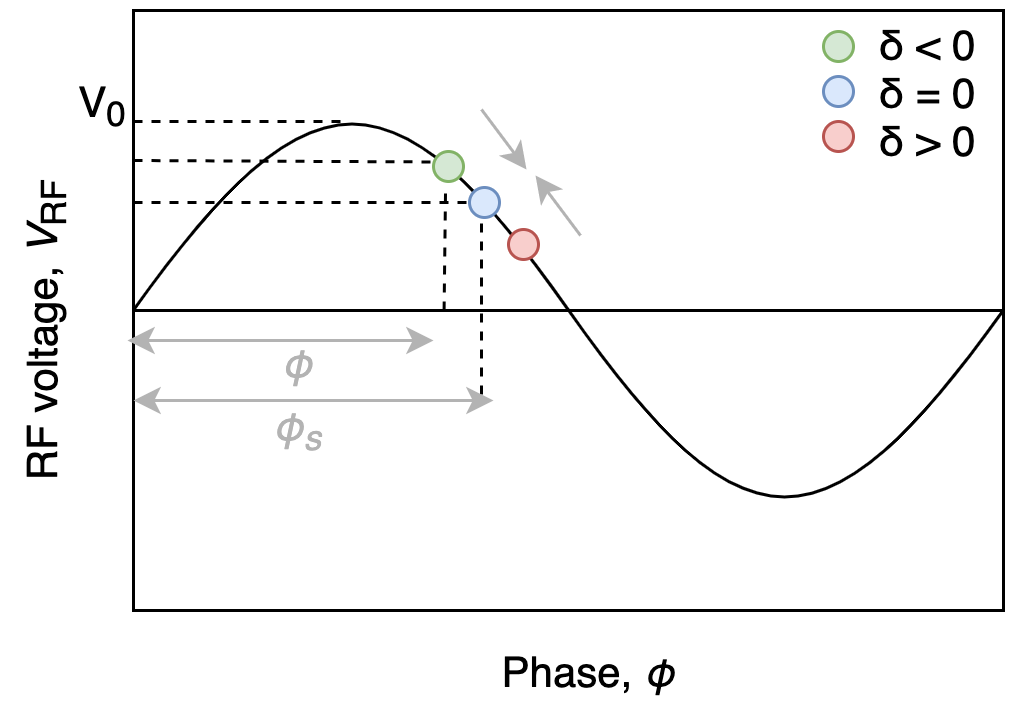
\includegraphics[width=0.6\textwidth]{images/Ch2/phase_focusing_synchrotron_motion.png}
        \caption{Phase stability for particles in a circular accelerator which operates above transition.}
        \label{fig:phase_focusing}
 \end{figure}

In particular, the non-synchronous particles oscillate around the phase of the synchronous particle performing synchrotron oscillations (similarly with the betatorn oscillations in the transverse plane). Turn-by-turn the particles perform oscillations around the phase of sunchronous paticle performing synchrotron oscillations. The equations of motion for a particle passing through a system of synchronised RF cavities located around the accelerator are~\cite{wolski2014}: % wolski p. 173 Eq.(5.53) and (5.54)
\begin{equation}\label{eq:long_eq_motion_z}
    z^\prime = - \eta_p \delta,
\end{equation}
\begin{equation}\label{eq:long_eq_motion_delta}
    \delta^\prime = - \frac{qV_\mathrm{RF}}{c p_0 C} \left ( \sin{\phi_s} - \sin{\left ( \phi_s - \frac{\omega_\mathrm{RF} z}{c} \right)} \right ),
\end{equation}
where $z^\prime = dz/ds$, $\delta^\prime = d\delta/ds$, $e$ is the charge of a proton, $c$ is the speed of light, $p_0$ is the reference momentum, $C$ is the circumference of the machine, $\omega_\mathrm{RF}$ is the angular frequency of the RF system, $\phi_s$ is the phase of the synchronous particle and $\eta_p$ is the phase slip factor.

The synchrotron tune, $Q_s$, is the number of synchrotron oscillations performed during one complete revolution around the machine and is computed as follows~\cite{wolski2014}: % Wolski Eq.(5.49) p. 170
\begin{equation}\label{eq:Qs} 
    Q_s = \frac{1}{2\pi}\sqrt{-\frac{e V_\mathrm{RF}}{c p_0} \frac{\omega_\mathrm{RF} C}{c} \eta_p \cos{\phi_s}},
\end{equation}
where $e$ the proton charge, $V_\mathrm{RF}$ the amplitude of the RF cavity voltage, $c$ the speed of light, $p_0$ the reference momentum, $\omega_\mathrm{RF}$ the angular frequency of the RF system and $\phi_s$ the synchronous phase.

\section{Collective effects}
Up to now, the motion of the particles was studied neglecting the interaction between them within the bunch. Collective effects in an accelerator are mechanisms that depend on the interaction of particles with each other e.g. beam-beam interactions, space sharge effects, wakefields, intra-beam scattering etc~\cite{Zimmermann:2264408}. The collective effects usually become crucial for high intensity beams as they can lead to instabilities which then may leed to beam losses degradig the beam quality and affecting the performance of the accelerator. The discussion here, is limited in the 


\subsection{Transverse beam impedance}\label{subsec:wakefields}
- clasic figure, equations, chao, tune shift and damping time. 
- see presentation from auth.

%\subsection{Active feedback?}
\section{Optics models of accelerators}
% or optics design
\subsection*{MADX}
Table with parameters for sps lattice, eg average beta function, tune etc. circumference, Q20 and Q26.

presentation AUTH?


See sondre's thesis for inspiration on the structure.
\section{General parameters of the studies}
% Maybe this should be mentioned at the end of project objectives and thesis outline.
% The following paragraphs are taken from the APR Ch.1.3 
\subsection{SPS optics}\label{subsec:SPS_optics_model}
 The studies presented in this thesis were performed for the nominal SPS optics for the LHC filling which are called Q26 optics as the higher integer part of the tune in both planes is 26. 

 \normalsize{\textbf{SPS nominal model}\\
 The model for the Q26 optics can be found in the official CERN repository~\cite{SPS_optics_repo} and will be referred to as the nominal SPS model in this thesis. The values of the optics parameters in what follows correspond to the model values unless stated otherwise.

 \normalsize{\textbf{SPS non-linear model}\\
\textcolor{red}{Move this section to chapter 6.}
The nominal SPS model includes only the nonlinear fields produced by the chromatic sextupoles. However, one of the most important sources of non-linearities in SPS are the odd multipole components of its main dipole magnets. For some of the studies presented in this thesis their impact on the beam dynamics must be studied and therefore they should be included in the nominal model. 

% APR Chapter 3.1
The multipole error of the SPS main dipoles are unfortunately not available from magnetic measurements. On this ground a non-linear optics model of the SPS has been established with beam-based measurements of the chromatic detuning over a range of momentum deviation~\cite{Carlà:2664976, Alekou:2640326}.  The optics model was obtained by assigning systematic multipole components to the main lattice magnets, in the nominal model of SPS, in order to reproduce the tune variation with themomentum deviation as it was measured in the real machine. The calculations were performed with MAD-X [].

The values of the multipole components up to seventh order obtained from this method are given in Table~\ref{tab:sps_mult_270GeV} where, ($b_3^A, b_3^B$) ($b_5^A, b_5^B$) and ($b_7^A, b_7^B$) stand for the sextupolar, decapolar and decatetrapolar mutipoles respectively. Note that different values have been obtained foreach of the two different kinds of SPS main dipoles (MBA and MBB) which are marked withthe indices A and B respectively.

\begin{table}[ht] % table take from the APR
    \caption{Multipole errors from SPS non-linear model, at 270\,GeV.} % title of Table
    \centering % used for centering table
    \begin{tabular}{c c c c} % centered columns (4 columns)
    \hline\hline %inserts double horizontal lines
    Multipole & Value  \\ [0.5ex] % inserts table
    %heading
    \hline  % inserts single horizontal line
    $b_3^A, b_3^B$ & 8.1 $\times 10^{-4}$\,$\mathrm{m^{-2}}$, 1.1 $\times 10^{-3}$\,$\mathrm{m^{-2}}$\\ 
    $b_5^A, b_5^B$ & 9.2\,$\mathrm{m^{-4}}$, $-$10\,$\mathrm{m^{-4}}$ \\
    $b_7^A, b_7^B$ & 1.3 $\times 10^{5}$\,$\mathrm{m^{-6}}$, 1.4 $\times 10^{5}$\,$\mathrm{m^{-6}}$\\ [1ex] % [1ex] adds vertical space
    \hline %inserts single line
    \end{tabular}
    \label{tab:sps_mult_270GeV} % is used to refer this table in the text
    \end{table}


\textbf{random multiple errros? } Like in APR.Ch.3.2.2.

\
\section{Wakefields and impedances}\label{sec:wakefields_theory}

he terms dipolar and quadrupolar have been chosen as the dipolar wake function acts on the test proton like a dipole magnet (the kick is the same whatever its transverse location), whereas the quadrupolar term acts like a quadrupole magnet (the kick increases linearly with the transverse offset of the test particle). Benoits thesis p.44


\section{Tracking simulation codes}\label{sec:simualtion_codes}
In this section the two tracking simulation codes used in this thesis to study the noise-induced emittance growth are presented. Both codes are macroparticle tracking libraries that simulate the particle motion in the six-dimensional (6D) phase space $(x, x^\prime, y, y^\prime, z, \delta)$. The first code performs tracking between interaction points around a circular accelerator with the use of trasnfer matrices while the second one uses the detailed optics model of the machine.

\subsection{PyHEADTAIL}\label{subsec:pyheadtail}

PyHEADTAIL~\cite{pyheadtail_repository} is an open-source 6D macroparticle tracking code, developed at CERN, which was originally designed to study collective effects in circular machines and to be easily extrensible with custom elements. 
% https://indico.cern.ch/event/930271/contributions/3910265/attachments/2066139/3467770/30June2020_Simulations_emit_growthCC_RFnoise.pdf  
Details on its implementation and its features can be find in Refs.~\cite{pyheadtail_manual_adrian, pyheadtail_schenk}. Below the main steps of a simulation are listed: % according to the interest of this thesis.

% Thesis david: https://cds.cern.ch/record/2707064/files/CERN-THESIS-2019-272.pdf (p.45) and for the transverse matrix.

\begin{enumerate}
    \item \textbf{Machine initialisation:} The accelerator ring is splitted into a number of segments of equal length, after each of which there is an interaction point (IP). At the interaction points the macroparticles experience kicks from various accelerator components (feedback system, multipoles etc) or from collective effects such as the wakefields. The machine parameters, such as the circumference, the betatron and synchrotron tunes and the optics at the interaction points are defined. It should be noted that PyHEADTAIL uses smooth approximation which means that only a few segments are defined per turn. % which results to a very  rough optics model.
    \item \textbf{Bunch initialisation:}  A particle bunch is represented by a collection of macroparticles, each of which represents a clustered collection of physical particles. Each macroparticle is described by four transverse $(x, x^\prime, y, y^\prime)$ and two longitudinal coordinates $(z, \delta)$, a mass and an electric charge. For the studies presented in this thesis $10^{5}$ macroparticles are sufficient for an accurate represantation of the bunch, unless it is stated otherwise. There are various distributions available. In this thesis the simulations are performed using a Gaussian distribution in transverse and longitudinal planes.
    \item \textbf{Transverse tracking}: In the transverse plane, the macroparticles are transported from one interaction point to another by linear transfer matrices which take into account the optics parameters at the beginning and the end of the corresponding segment. For example, in the horizontal plane the transport of each macroparticle from IP1 to IP2 along the ring is given by:
    \begin{equation}
        \binom{x_i}{x_i^\prime}_{\mathrm{IP0}} = M \binom{x_i}{x_i^\prime}_{\mathrm{IP1}},
    \end{equation}
    where $i=1, ..., N$ with N being the number of macroparticles and the matrix $M$ is given by:
    \begin{equation}\label{eq:linear_transfer_map}
        M = \begin{pmatrix}
            \sqrt{\beta_{x, \mathrm{IP0}}} & 0 \\ 
            -\frac{\alpha_{x, \mathrm{IP0}}}{\sqrt{\beta_{x,  \mathrm{IP0} }}} & \frac{1}{\sqrt{\beta_{x, \mathrm{IP0}}}}
            \end{pmatrix} \begin{pmatrix}
                \cos(\Delta \mu_{x, \mathrm{IP0 \to IP1 }}) & \sin(\Delta \mu_{x, \mathrm{IP0 \to IP1 }})\\
                 - \sin(\Delta \mu_{x, \mathrm{IP0 \to IP1 }})  &\cos(\Delta \mu_{x, \mathrm{IP0 \to IP1 } }) 
                \end{pmatrix}  \begin{pmatrix}
                    \sqrt{\beta_{x, IP1}} & 0 \\ 
                    -\frac{\alpha_{x, IP1}}{\sqrt{\beta_{x, IP1}}} & \frac{1}{\sqrt{\beta_{x, IP1}}}
                    \end{pmatrix} 
    \end{equation}
    where $\alpha_{x, \mathrm{IP0/IP1}}$ and $\beta{x, \mathrm{IP0/IP1}}$ are the optics paramters at the interaction points IP0 and IP1 respectively and $\Delta \mu_{x, \mathrm{IP0 \to IP1 }}$ the phase advance from IP0 to IP1. As smooth approximation is used, the phase advance equals: 
    \begin{equation}\label{eq:phase_advance_smooth_approximation}
        \Delta \mu_{x, \mathrm{IP0 \to IP1 }} = Q_x \frac{L}{C},
    \end{equation}
    where $Q_x$ is the horizontal betatron tune, $C$ the machine circumference and $L$ the length of the corresponding segment. It should be noted that if no detuning source is added (see next step) the matrix $M$ is the same for all particles.
    \item \textbf{Chromaticity and detuning with transverse amplitude:} The chromaticity (up to higher orders) and amplitude detuning are implemented as a change of the phase advance of each individual particle as follows (example for the horizontal plane):
    \begin{equation}\label{eq:change_phase_advance_detunign}
        \Delta \mu_{x, i \mathrm{IP0 \to IP1 }} = \Delta \mu_{x, \mathrm{IP0 \to IP1 }} + (\xi^{1}_x \delta_i + \alpha_{xx}J_{x, i} + \alpha_{xy}J_{y,i}) \frac{\Delta \mu_{x, \mathrm{IP0 \to IP1 }}}{2\pi Q_x}, 
    \end{equation}
    where $i=1, ..., N$ with N being the number of macroparticles, $\Delta \mu_{x, \mathrm{IP0 \to IP1 }}$ is the phase advance for all macroparticles defined in the previous step, $\xi_x^{1}$ the horizontal chromaticity of first order normalised to the tune $\alpha_{xx}$ and $\alpha_{xy}$ are the detuning coefficients, while $J_x$ and $J_y$ are the horizontal and vertical actions of the macroparticle. Therefore, in the presence of detuning the elements of the $M$ matrix are different for every particle.

    \item \textbf{Longitudinal tracking:}  In PyHEADTAIL the longitudinal particle dynamics are described with the longitudinal equations of motion (ref to eq earlier.) % slide 37: https://www2.kek.jp/accl/legacy/seminar/file/PyHEADTAIL_PyECLOUD_2.pdf 
    The longitudinal coordinates are advanced once per turn after solving numerically the equations of motion~\cite{pyheadtail_schenk}. The motion can be linear or not (non-linear RF system). The studies presented in this thesis use the linear longitudinal tracking.

    \item \textbf{Trasnverse impedance effects:} In PyHEADTAIL, wakefield kicks are used to implement the effect of the transverse impedance in time domain. To improve the computational efficiency, the total impedance of the full machine is lumped in one of the interaction points along the ring and the kicks are applied on the macroparticles once per turn. Additionally, instead of computing the wakefield kicks from each particle to the rest individually, the bunch is divided in a number of longitudinal slices and the macroparticles in each slice recieve a wakefield kick generated by the preceding slices\footnote{This is valid in the ultrarelativistic scenario when no wakefield is generated in front of the bunch. The condition applies for the SPS experiments described in this thesis, performed at 270\,GeV.}~\cite{Salvant:1274254}. This is illustrated schematically in Fig.~\ref{fig:longitudinal_slicing_wakefields}. A large number of slices is required such as the wakes can be assuemed constant within the slice. A high number of macroparticles is also needed in order to avoid statistical noise effects caused by undersampling~\cite{pyheadtail_manual_adrian}. For the studies presented in 500 slices are used over a range of three rms bunch lengths in both directions from the bunch center with the bunch being represented by $10^6$ macroparticles (instead of $10^5$ required for simulations without impedance effects).
    

    \begin{figure}[!ht]
        \centering
        \begin{subfigure}[t]{0.45\textwidth}
            \centering
            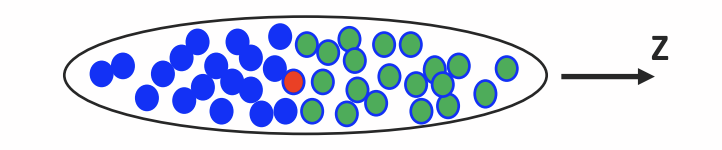
\includegraphics[width=1\textwidth]{images/Ch2/before_slicing.png}
            \caption{Without slicing}
            %\label{fig:add_label_here}
        \end{subfigure}
        \hfill
        \begin{subfigure}[t]{0.45\textwidth}
            \centering
            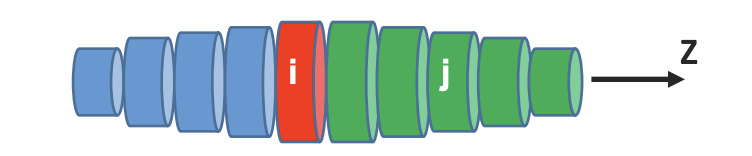
\includegraphics[width=1\textwidth]{images/Ch2/after_slicing.png}
            \caption{With slicing}
            %\label{fig:add_label_here}
        \end{subfigure}
        \hfill
         \caption{Longitudinal bunch slicing for the implementation of wakefields kicks in PyHEADTAIL. Without the slicing technique (left) the wake kicks on the red macroparticle are generated from all the green macroparticles resulting to computationally heavy simulations. Instead, when the bunch is sliced longitudinally (right) the wake kicks on the macroparticles in the red slice $i$ are generated by the macroparticles in the green slices $j$, decreasing significantly the computation time. The figures are a courtesy of M. Schenk~\cite{pyheadtail_schenk}} % bunch passage
         \label{fig:longitudinal_slicing_wakefields}
     \end{figure}
        
    The wakefield kicks are computed using a convolution of the wake function with the moments of each particle. %p.39 michael schenk thesis
    The wake functions are available from detailed imepdance model of the machine which are obtained from a combination of theoretical computations, electromagentic simulations and can be imported in PyHEADTAIL in form of tables. More details on the SPS impedance model are provided in Section~\ref{sec:sps_impedance_model}.
    
    \item \textbf{Data acquisition:} The updated bunch coordinates after each turn are available at IP0 for post processing. Typically, $10^{5}$ turns are required for the noise-induced emittance growth simulation presented in this thesis. 
    
\end{enumerate}


%Last sentence from (LinearMap): https://github.com/PyCOMPLETE/PyHEADTAIL/blob/master/PyHEADTAIL/trackers/longitudinal_tracking.py
%or longutidanl equations of motion: slide 37 https://www2.kek.jp/accl/legacy/seminar/file/PyHEADTAIL_PyECLOUD_2.pdf

Figure~\ref{fig:pyheadtail_accelerator_model} shows a graphic representation of the accelerator model and the tracking procedure supporting the steps described above.
% Graph is created app.diagrams.net and is saved in goodle dirve.

\begin{figure}[!h]
    \centering         
    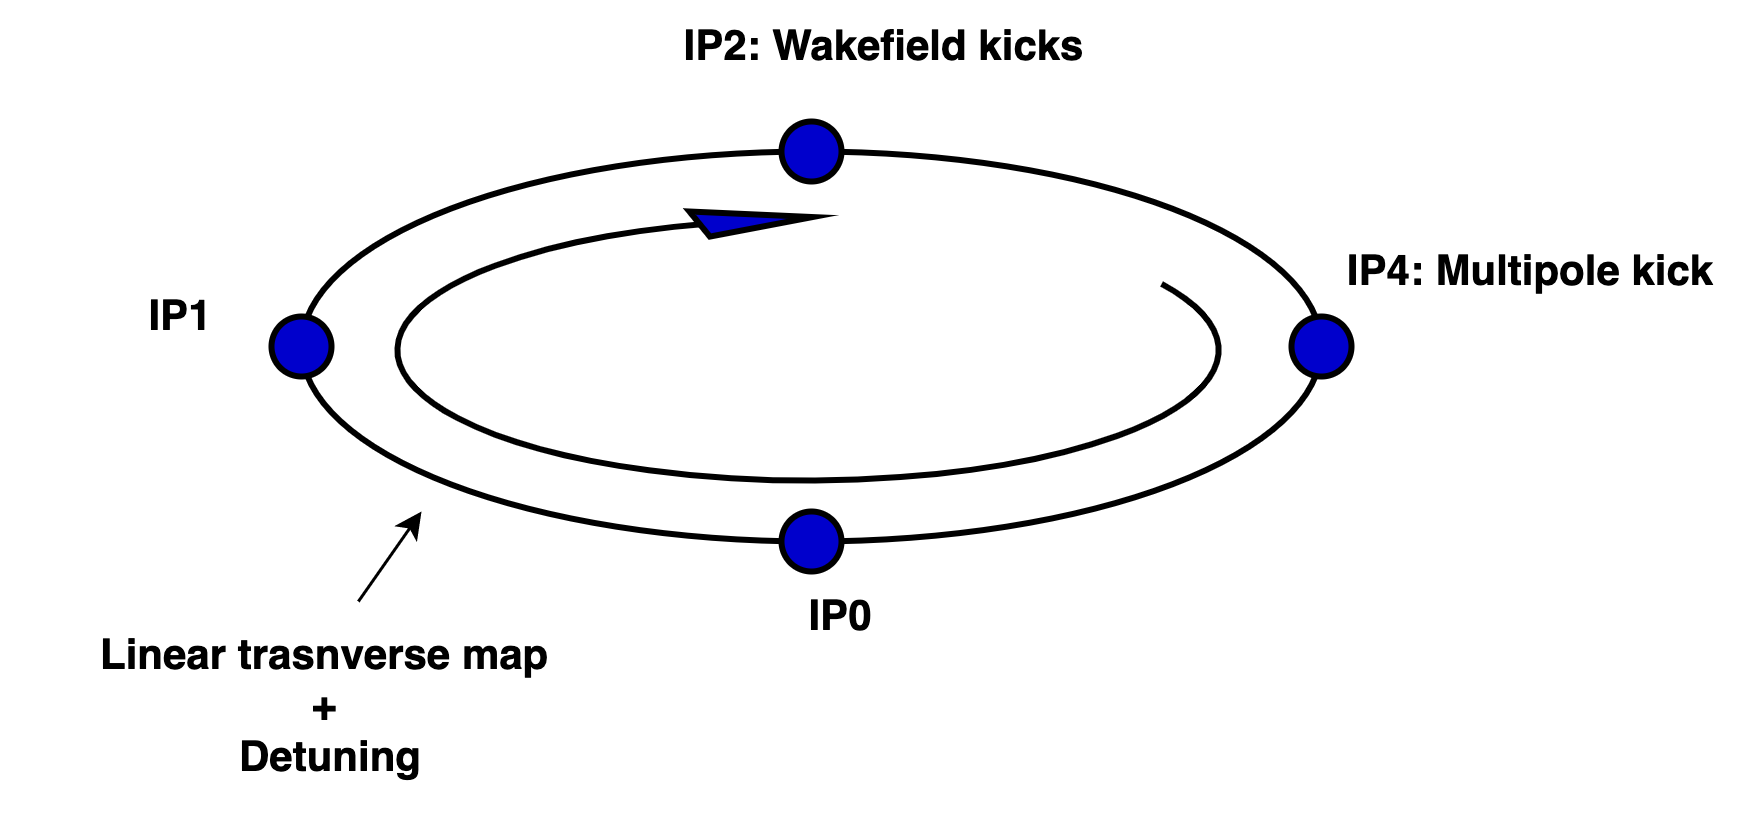
\includegraphics[width=0.6\textwidth]{images/Ch2/accelerator_model_graph_pyheadtail.png}
        \caption{Graphic represantation of the accelerator model and tracking procedure in PyHEADTAIL (inspered by the graphs in Refs.~\cite{pyheadtail_schenk, inproceedings_ibs_pyheadtail}). In this example the ring is splitted in four segments seperated by the interaction points (IPs). Wakefield and mulitple kicks are applied on the macroparticles in IP2 and IP4. The macroparticles are transported between the IPs by a linear map (which can include detuning effects) in the transverse plane.  The longitudinal coordinates are updated once per turn without being visualised in this plot.}
        \label{fig:pyheadtail_accelerator_model}
 \end{figure}


\subsection{Sixtracklib}\label{subsec:sixtracklib}
%Introduction to sixtrackib: https://indico.cern.ch/event/833895/contributions/3577803/attachments/1927226/3190636/intro_sixtracklib.pdf
% https://inspirehep.net/files/6273430c727ace3796a92d069f651ade


Check a presentation from kostas.